\documentclass[12pt,twoside]{article}
%%%%%%%%%%%%%%%%%%%%%%%%%%%%%%%%%%%%%%%%%%%%%%%%%%%%%%%%%%%%%
% Meta informations:
\newcommand{\trauthor}{Jan Fabian Schmid}
\newcommand{\trtype}{Seminar Paper} %{Seminararbeit} %{Proseminararbeit}
\newcommand{\trcourse}{Knowledge Processing}
\newcommand{\trtitle}{Examination of a framework for multi-objective analysis of computational models}
\newcommand{\trmatrikelnummer}{6440383}
\newcommand{\tremail}{2schmid@informatik.uni-hamburg.de}
\newcommand{\trarbeitsbereich}{Knowledge Technology, WTM}
\newcommand{\trdate}{10.11.2015}

%%%%%%%%%%%%%%%%%%%%%%%%%%%%%%%%%%%%%%%%%%%%%%%%%%%%%%%%%%%%%
% Languages:

% Falls die Ausarbeitung in Deutsch erfolgt:
% \usepackage[german]{babel}
% \usepackage[T1]{fontenc}
% \usepackage[latin1]{inputenc}
% \usepackage[latin9]{inputenc}	 				
% \selectlanguage{german}

% If the thesis is written in English:
\usepackage[english]{babel} 						
\selectlanguage{english}

%%%%%%%%%%%%%%%%%%%%%%%%%%%%%%%%%%%%%%%%%%%%%%%%%%%%%%%%%%%%%
% Bind packages:
\usepackage{acronym}                    % Acronyms
\usepackage{algorithmic}								% Algorithms and Pseudocode
\usepackage{algorithm}									% Algorithms and Pseudocode
\usepackage{amsfonts}                   % AMS Math Packet (Fonts)
\usepackage{amsmath}                    % AMS Math Packet
\usepackage{amssymb}                    % Additional mathematical symbols
\usepackage{amsthm}
\usepackage{booktabs}                   % Nicer tables
%\usepackage[font=small,labelfont=bf]{caption} % Numbered captions for figures
\usepackage{color}                      % Enables defining of colors via \definecolor
\definecolor{uhhRed}{RGB}{254,0,0}		  % Official Uni Hamburg Red
\definecolor{uhhGrey}{RGB}{122,122,120} % Official Uni Hamburg Grey
\usepackage{fancybox}                   % Gleichungen einrahmen
\usepackage{fancyhdr}										% Packet for nicer headers
%\usepackage{fancyheadings}             % Nicer numbering of headlines

%\usepackage[outer=3.35cm]{geometry} 	  % Type area (size, margins...) !!!Release version
%\usepackage[outer=2.5cm]{geometry} 		% Type area (size, margins...) !!!Print version
%\usepackage{geometry} 									% Type area (size, margins...) !!!Proofread version
\usepackage[outer=3.15cm]{geometry} 	  % Type area (size, margins...) !!!Draft version
\geometry{a4paper,body={5.8in,9in}}

\usepackage{graphicx}                   % Inclusion of graphics
%\usepackage{latexsym}                  % Special symbols
\usepackage{longtable}									% Allow tables over several parges
\usepackage{listings}                   % Nicer source code listings
\usepackage{multicol}										% Content of a table over several columns
\usepackage{multirow}										% Content of a table over several rows
\usepackage{rotating}										% Alows to rotate text and objects
\usepackage[hang]{subfigure}            % Allows to use multiple (partial) figures in a fig
%\usepackage[font=footnotesize,labelfont=rm]{subfig}	% Pictures in a floating environment
\usepackage{tabularx}										% Tables with fixed width but variable rows
\usepackage{url,xspace,boxedminipage}   % Accurate display of URLs
\usepackage{wrapfig}
%%%%%%%%%%%%%%%%%%%%%%%%%%%%%%%%%%%%%%%%%%%%%%%%%%%%%%%%%%%%%
% Configurationen:

\hyphenation{whe-ther} 									% Manually use: "\-" in a word: Staats\-ver\-trag

%\lstloadlanguages{C}                   % Set the default language for listings
\DeclareGraphicsExtensions{.pdf,.svg,.jpg,.png,.eps} % first try pdf, then eps, png and jpg
\graphicspath{{./src/}} 								% Path to a folder where all pictures are located
\pagestyle{fancy} 											% Use nicer header and footer

% Redefine the environments for floating objects:
\setcounter{topnumber}{3}
\setcounter{bottomnumber}{2}
\setcounter{totalnumber}{4}
\renewcommand{\topfraction}{0.9} 			  %Standard: 0.7
\renewcommand{\bottomfraction}{0.5}		  %Standard: 0.3
\renewcommand{\textfraction}{0.1}		  	%Standard: 0.2
\renewcommand{\floatpagefraction}{0.8} 	%Standard: 0.5

% Tables with a nicer padding:
\renewcommand{\arraystretch}{1.2}

%%%%%%%%%%%%%%%%%%%%%%%%%%%%
% Additional 'theorem' and 'definition' blocks:
\theoremstyle{plain}
\newtheorem{theorem}{Theorem}[section]
%\newtheorem{theorem}{Satz}[section]		% Wenn in Deutsch geschrieben wird.
\newtheorem{axiom}{Axiom}[section] 	
%\newtheorem{axiom}{Fakt}[chapter]			% Wenn in Deutsch geschrieben wird.
%Usage:%\begin{axiom}[optional description]%Main part%\end{fakt}

\theoremstyle{definition}
\newtheorem{definition}{Definition}[section]

%Additional types of axioms:
\newtheorem{lemma}[axiom]{Lemma}
\newtheorem{observation}[axiom]{Observation}

%Additional types of definitions:
\theoremstyle{remark}
%\newtheorem{remark}[definition]{Bemerkung} % Wenn in Deutsch geschrieben wird.
\newtheorem{remark}[definition]{Remark} 

%%%%%%%%%%%%%%%%%%%%%%%%%%%%
% Provides TODOs within the margin:
\newcommand{\TODO}[1]{\marginpar{\emph{\small{{\bf TODO: } #1}}}}

%%%%%%%%%%%%%%%%%%%%%%%%%%%%
% Abbreviations and mathematical symbols
\newcommand{\modd}{\text{ mod }}
\newcommand{\RS}{\mathbb{R}}
\newcommand{\NS}{\mathbb{N}}
\newcommand{\ZS}{\mathbb{Z}}
\newcommand{\dnormal}{\mathit{N}}
\newcommand{\duniform}{\mathit{U}}

\newcommand{\erdos}{Erd\H{o}s}
\newcommand{\renyi}{-R\'{e}nyi}
%%%%%%%%%%%%%%%%%%%%%%%%%%%%%%%%%%%%%%%%%%%%%%%%%%%%%%%%%%%%%
% Document:
\begin{document}
\renewcommand{\headheight}{14.5pt}

\fancyhead{}
\fancyhead[LE]{ \slshape \trauthor}
\fancyhead[LO]{}
\fancyhead[RE]{}
\fancyhead[RO]{ \slshape \trtitle}

%%%%%%%%%%%%%%%%%%%%%%%%%%%%
% Cover Header:
\begin{titlepage}
	\begin{flushleft}
		Universit\"at Hamburg\\
		Department Informatik\\
		\trarbeitsbereich\\
	\end{flushleft}
	\vspace{3.5cm}
	\begin{center}
		\huge \trtitle\\
	\end{center}
	\vspace{3.5cm}
	\begin{center}
		\normalsize\trtype\\
		[0.2cm]
		\Large\trcourse\\
		[1.5cm]
		\Large \trauthor\\
		[0.2cm]
		\normalsize Matr.Nr. \trmatrikelnummer\\
		[0.2cm]
		\normalsize\tremail\\
		[1.5cm]
		\Large \trdate
	\end{center}
	\vfill
\end{titlepage}

	%backsite of cover sheet is empty!
\thispagestyle{empty}
\hspace{1cm}
\newpage

%%%%%%%%%%%%%%%%%%%%%%%%%%%%
% Abstract:

% Abstract gives a brief summary of the main points of a paper:
\section*{Abstract}
  Your text here...

% Lists:
\setcounter{tocdepth}{2} 					% depth of the table of contents (for Seminars 2 is recommented)
\tableofcontents
\pagenumbering{arabic}
\clearpage

%%%%%%%%%%%%%%%%%%%%%%%%%%%%
% Content:

% the actual content, usually separated over a number of sections
% each section is assigned a label, in order to be able to put a
% crossreference to it

\section{Introduction}
\label{sec:introduction}

\subsection{Problem}
The studied paper \cite{doncieux2015multi} tries to cover the problems arising at the use of sophisticated computational models.
In more and more areas computational models are used for increasingly hard scientific issues.
Doncieux et al. break the problem down to the epistemic opacity. Which they define as follows:
\begin{align*}
	&\text{\textit{A process is epistemically opaque relative to a cognitive agent X at time t just in}}\\
	&\text{\textit{case X does not know at t all of the epistemically relevant elements of the process.}}
\end{align*}
Thus epistemic opacity is a term to describe the state of knowledge of an agent in matters of a specific process at a specific point in time.
It says that the agent has not recognized the process in its entirety at the point in time.
In case of computational methods the term can be used to describe a situation in which a scientist developed a complex model, to study an even more complex process, during the simulation of the model he is however not aware which model parameters are interesting to use since the model is too complex to know the implications of different parameter values. This holds for the time until he finally studied the model in an extent that allows him to predict the effects of changed parameter values.\medskip

Epistemic opacity may stem from a complicated mathematical foundation to the model, from the complex interaction of different model parts with each other or from the effect of different input-parameters.
They say: \glqq[...], the computational model is in itself a complex system to study in order to unravel its unforeseen features\grqq{} \cite{doncieux2015multi} p. 3.
This problem can lead to an extensive search in parameter space for the \glqq best\grqq{} parameter values.
The researcher might have an intuition for some good parameter values, but these are biased by his assumptions about the model. 

Furthermore in a complex system it might not be obvious what properties of the model are actually desirable. Hence the \glqq best\grqq{} model parameters wouldn't be recognized if found.
Since the model should lead to novel knowledge, and proven or disproven assumptions about the modelled system, interesting parameter-sets for further studying are desired. Interesting parameters should be somehow different from other parameters and state something about the model.

To overcome the epistemic opacity the researcher would have to analyse the complex model by approximating it with a model again (cf. \cite{doncieux2015multi} p. 3). This process of modelling a modell could be repeated multiple times, each step using a more abstract and simple model, until it is easy enough to understand by the researcher. The knowledge gained from the simpler models could then be used to understand the more complex models. At some point the problem is understood well enough to use the primary model with confident insight.

\subsection{Suggested solution}
Because modelling a model becomes exponentially intricate and success isn't guaranteed it can hardly be a feasible approach to study a problem. The paper suggests to exploit the fact, that the computational model can be computed in a \glqq huge number of experiments\grqq{} \cite{doncieux2015multi} p. 3.
They suggest a framework method that once set up searches automatically for interesting model parameters, which can then be analysed.
The framework requires that a set of functions that describe the model with three properties are given:
\begin{enumerate}
	\item The functions measure the model performance.
	\item For optimal model performance the functions have to be maximized or minimized.
	\item Some functions are contrary to each other, as optimizing one function value worsens an other.
\end{enumerate}
The given function set maps parameter space to behaviour space. Calculating many possible solutions allows to find relations between both spaces.
Since the performance of individual functions is contrary to each other multi-objective algorithms can be used to find sets of trade-off solutions (cf. \cite{doncieux2015multi} p. 3).
Doncieux et al. then suggest to use evolutionary multi-objective algorithms, since they are efficient and versatile in usage. Following the steps of the framework interesting parameter sets are thereby found.
The paper suggests then some tools to acquire knowledge about the implications of obtained parameter values on model behaviour.\\
It is important to note that the proposed method is not used to find the best parametrisation for optimal model performance, but to aquire knowledge about the behaviour of the model for different parameter values \footnote{cf. \cite{doncieux2015multi} p. 9}.

\subsection{Goals and structure of this paper}
This paper is supposed to give an in-depth analysis of the presented paper \cite{doncieux2015multi}.
In Chapter \ref{sec:background} some background, necessary to understand the main concepts of the paper, will be given.
The proposed frame work of Doncieux et al. will then be presented in a summarized form in Chapter \ref{sec:model}.
In the following chapter \ref{sec:analysis} the model and its results will be critically reviewed.
Especially the applicability of and assumptions made by the framework will be discussed.
Chapter \ref{sec:concl} will conclude the paper by stating the achieved insights on the usage and applicability of the framework. 
%- Is this framework applicable to all kinds of computational methods? What conditions must be met by the computational method?
\section{Background Information}
\label{sec:background}
The crucial concepts to understand the framework for computational methods are presented in this chapter.

At first the topics of Multi-objective problems and what a optimal solution to such an ambiguous problem looks like are outlined. These issues will be discussed in section \ref{back:multi-opt}. 
The functionality of evolutionary algorithms is subject to section \ref{back:evo}.
Section \ref{back:evo_in_multi-opt} brings these concepts in context for the usage of evolutionary algorithms in Multi-objective-optimization.
And finally in section \ref{back:indicators} some indicators are introduced, that will be used to analyse the results of multi-objective optimization.

\subsection{Multi-objective optimization}
\label{back:multi-opt}
%\cite{miettinen2012nonlinear}\\
Doncieux et al. \cite{doncieux2015multi} formalize optimization problems approximately as follows:

\begin{align*}
	\text{Find the parameter }\textbf{X} &=
	\left \{
	\begin{tabular}{c}
		$x_1$\\
		$x_2$\\
		\vdots\\
		$x_m$
	\end{tabular}
	\right \}
	\in \mathbb{R}^m \text{that maximizes (or minimizes) f(\textbf{X}) under}\\
		 \text{a given set of constraints.}
\end{align*}

For $m = 1$ such a task is called mono-objective problem, whereas it's a multi-objective problem for any $m > 1$.

As soon as you want to examine a real world like problem it's very likely that the solution won't be a single one dimensional value. Instead there will be multiple objectives to be considered simultaneously.
Fonseca and Fleming state that an optimal solution to a multi dimensional problem is commonly not optimal for each of the objectives (cf. \cite{fonseca1995overview} p. 1)
This should be the case as long as the different objectives are somehow conflicting.
They say further that you would rather aim at a solution that is at least acceptable for all sub-objectives.
This however isn't a explicit problem statement. In a non-trivial case there will be several quite different alternative approaches to the problem that are optimal in some aspects.
All these approaches should be valid solutions given by a multi-objective optimization-algorithm.
To allow this to happen the \textbf{Pareto dominance} relation and the \textbf{Pareto-optimal set} are introduced.
A solution $\mathbf{X_1}$ dominates another solution $\mathbf{X_2}$ if $\mathbf{X_1}$ is not worse than $\mathbf{X_2}$ for any objective and for at least one objective strictly better (cf. \cite{doncieux2015multi} p. 6).
A solution is called Pareto-optimal if it isn't dominated. All Pareto-optimal solutions form the Pareto-optimal set. 
Since the Pareto dominance relation is a partial ordering it allows any number of optimal solutions.
The Pareto-optimal set contains interesting solutions, because each of its members is a solution that is best in some aspect.

\subsection{Evolutionary algorithms}
\label{back:evo}
An evolutionary algorithm is a stoachastical approach to obtain a solution to a problem. Because of the stochastic behavior in general the solutions won't be optimal, but are often feasible. Similar to the evolutionary process in nature, a group of individuals is developed over multiple generations under the influence of a pressure to adapt to the environment. An induviduum during this process represents a solution to the problem.\medskip

\begin{wrapfigure}{r}{0.3\textwidth}
	\begin{center}
		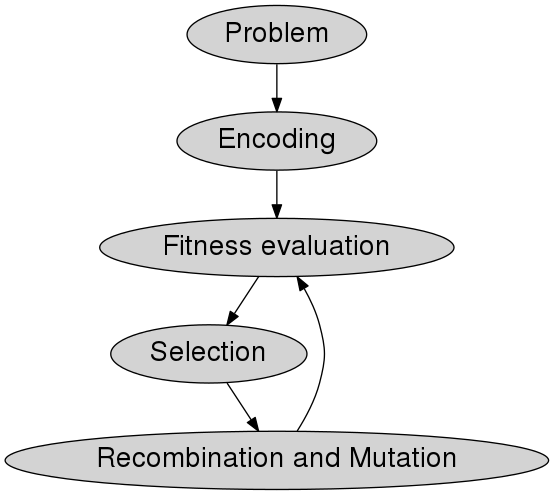
\includegraphics[height=.4\textwidth]{Bilder/evo.png}
	\end{center}
	\caption{General schemata of an evolutionary algorithm}
	\label{fig:evo}
\end{wrapfigure}

In figure \ref{fig:evo} a rough schemata of the important steps of an evolutionary algorithm are shown. At first an (genetic) encoding for all possible solutions to the problem has to be defined in a way that the different functions of the following steps can handle. The first group of solutions has to be initiated randomly.\\

Now the following steps are used repeatetly until some stopping criterea holds true:
\begin{enumerate}
	\item \textbf{Fitness evalution:} For each individual a \textbf{fitness function} evaluates its performance at solving the problem.
	\item \textbf{Selection}: Select the surviving invividuals, maybe just the best x\% of solutions. Some of the survivors are selected as parents for a new generation of individuals. For example a few percent of individuals with the highest fitness score are selected and with probability according to their fitness some more.
	\item \textbf{Recombination and Mutation:} New solutions are bred out of the selected parents through crossover and mutation.
\end{enumerate}

Such an simple evolutionary algorithm has only local convergence and therefore depends on the random initiation, as it follows a greedy approach, which follows the best solutions in a narrow seach space around the already avaiable solutions.

\subsection{Evolutionary algorithms for multi-objective optimization}
\label{back:evo_in_multi-opt}
As common optimization-algorithms like gradient descent or simulated annealing aren't suited to deal with multi-objective problems (cf. \cite{fonseca1995overview} p. 2) other approaches have been used.
One of the strengths evolutionary algorithms have, is to pursue different possible solutions at the same time. That's because in a well structured evolutionary algorithm the surviving individuals aren't only associated to the single best solution at the given time, but also momentary suboptimal solutions are being tracked.
Through crossover partially optimal parts of solutions can be exchanged as a whole. 
Therefore the Pareto front, the current Pareto optimal set during execution of the algorithm, can be explored effectively.

As evolutionary algorithms impose no mathematical constraints on the examined problem. The stochastic approach of evolutionary algorithms however entails to calculate many possible solutions in application to work properly. Also evolutionary algorithms don't ensure to find global optima, instead it converges to some local optimum. Accordingly only an approximation to the Pareto optimal solutions will be found.

The concept used by Doncieux et al. to gain knowledge about a system by analysing the results of a multi-objective optimization algorithm on it is called INNOVIZATION as they state this stands for 'INNOVation through optimIZATION' (cf. \cite{doncieux2015multi} p. 5).
Evolutionary multi-objective optimization algorithms were already used successfully with this approach as shown in \cite{efstratiadis2010one}, where Efstratiadis and Koutsoyiannis sum up the experience with the INNOVIZTION method for calibration of hydrological models.

\subsection{Indicators for multi-objective analysis}
\label{back:indicators}
To be able to analyse the gained information from multi-objective optimization on the examined problem Doncieux et al. introduce some indicators (cf. \cite{doncieux2015multi} p. 7 et seq.)
In the following it is without loss of generality assumed, that all objective-functions are to be maximized to be optimal.
The evolutionary multi-objective optimization is used multiple times on the problem. Each run generates a set of approximations to the Pareto optimal solutions called $\chi_i$ for the $i$-th run.
The required indicators are defined as follows.
\begin{itemize}
	\item The attainment function $\alpha_\chi(z)$ returns the probability to find in the set of results $\chi$ \textbf{at least one} solution $x$ that attains $z$, which means here that $x$ dominates $z$. This function can't be computed directly, but it can be approximated with the empirical attainment function $\alpha_r(z)$ over $r$ sets of approximation results as mean number of sets in which a solution is found that dominates $z$.
	\item The attainment surface $\Psi_p$ to an attainment function value $p$ is defined as the hyper surface in behaviour space over points with probability $p$ given by the attainment function.
	Therefore the 0-attainment surface $\Psi_0$ covers the set of non-dominated solutions and the 1-attainment surface $\Psi_0$ represents the worst performing solutions that will certainly be dominated.
	\item The hypervolume indicator $I^p_H(\chi)$ is defined for a particular reference point $p$ for a set of results $\chi_0$. A simplified attainment function $\beta\chi(z)$ definition is used for the hypervolume indicator, it returns $1$ if there is a solution in $\chi$, that dominates z, and $0$ otherwise. The hypervolume indicator is then defined as:
	\begin{align*}
		I^p_H(\chi_0) &= \int_{\psi_p}\beta\chi(z) dz
	\end{align*}
	With $\psi_p$ containing all points, that are equal or greater than $p$ in every dimension.
	Therefore $I^p_H(\chi)$ measures the area of points above $p$ that are dominated by a solution in $\chi$.
	In figure \ref{fig:attainment} a visualisation of the simplified attainment function and its hyper volumne is shown.
	\item The nadir $\eta(\chi)$ is the point with the least possible value for each objective found in $\chi$. So for each dimension all solutions in $\chi$ are scanned for the minimum value.
	When $\eta^i(\chi)$ is the nadir point to the $i$-th set of solutions, the conservative nadir point $\bar{\eta}$ is defined over $r$ sets of solutions and its values are the maximum value for each dimension found in any $\eta^i(\chi)$ with $i\in r$. The conservative nadir helps to get rid of outliers and is a more reliable representation of the \glqq worst\grqq{} returned solution.
\end{itemize}
 \addtocounter{footnote}{-1}
\begin{figure}[h]
	\begin{center}
		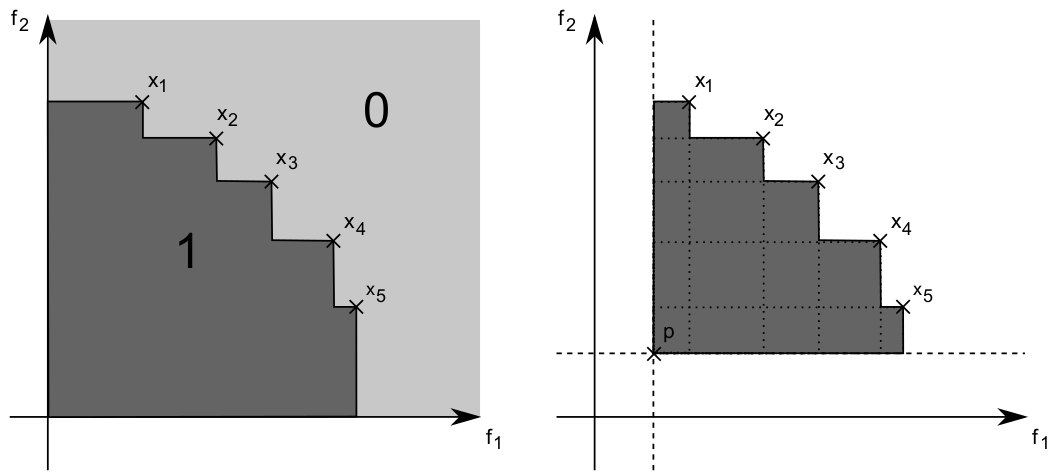
\includegraphics[width=1\textwidth]{Bilder/attainment.png}
	\end{center}
	\caption[f1 and f2 are the two objective functions in this example. On the left: $\beta\chi(z)$ for $\chi = \text{\{x1,x2,x3,x4,x5\}}$ and the attainment surfaces $\Psi_0$ and $\Psi_1$ (to the simplified attainment function $\beta$) are highlighted. On the right: The hypervolumne $I^p_H(\chi)$ is shown.]{f1 and f2 are the two objective functions in this example. On the left: $\beta\chi(z)$ for $\chi = \text{\{x1,x2,x3,x4,x5\}}$ and the attainment surfaces $\Psi_0$ and $\Psi_1$ (to the simplified attainment function $\beta$) are highlighted. On the right: The hypervolumne $I^p_H(\chi)$ is shown. \footnotemark}
	\label{fig:attainment}
\end{figure}
\footnotetext{image from \cite{doncieux2015multi} p. 8}
\paragraph{Summary:}
\textit{
	In this chapter the basics concepts used by the framework were introduced.
	The core part of the framework is a multi-objective optimization. 
	As shown the evolutionary approach is suitable for this task, its only drawback is the need for calculation of many iterations since there is no global convergence guaranteed.
	At last a couple of indicators for analysis of the obtained approximations of Pareto-optimal solutions were presented.
}

\section{Framework description and application}
\label{sec:model}
The proposed framework by Doncieux et al. \cite{doncieux2015multi} aims at automatically finding parameter values worth to be studied further.
There are three steps to application of the framework.
\begin{enumerate}
	\item The definition of functions to evaluate the performance of the examined computational method.
	\item Obtain an approximation of the Pareto optimal solutions by application of evolutionary multi-objective optimization.
	\item Knowledge creation by analysing the solutions.
\end{enumerate}
These steps are specified more in detail in the following sections.

\subsection{Search space and objective functions}
First the search space as part of the parameter space must be defined. For a set of $m$ unbound parameters $\in \mathbb{R}$ it would be $\mathbb{R}^m$. 

The framework relies on the comparison of different Pareto optimal solutions to find interesting parameter values, therefore multiple contrary objective functions have to be defined.
They need to be contrary in terms of not linearly dependent, since such a dependency would lead to a set of Pareto optimal solutions with only one member that is optimal for each objective function.
A simple second objective for a computational model whose performance actually only depends on a single one might be found in the computational cost.
With increasing computation time the algorithm might find better and better solutions. The optimal parameters would then be a compromise between quality of solution and time consumption.

\subsection{Application of multi-objective optimization}
If ideally no promising parameter vectors shall be missed it is important to make a dense search in parameter space, otherwise behaviours that only occur in a small area in parameter space might be skipped.
As explained in chapter \ref{back:evo_in_multi-opt} evolutionary algorithms are a good choice for the multi-objective-optimization.
The local convergence of evolutionary algorithms makes it necessary to run the optimization many times to ensure statistical significance of the results. Therefore the \textbf{first step} of application is to repeat the multi-objective optimization several times.
However the results from evolutionary algorithms strongly depend on their parametrisation, it is important to verify the results somehow.
Therefore the variability of results to successive runs of evolutionary multi-objective optimization can be checked.
%Similar results of most instances of the evolutionary algorithm hints at a convergence to a good approximation of the Pareto optimal set, whereas 
A high variability in results might be a sign of a ill parametrisation, as mentioned by Doncieux et al. (cf. \cite{doncieux2015multi} p. 11).
Thus the \textbf{second step} of application is the evaluation of disparity between multiple iterations of the algorithm. Doncieux et al. propose the following schemata for this:
\begin{enumerate}
	\item Compute the 0-attainment $\Psi_0$ and 1-attainment $\Psi_1$ surface.
	\item Calculate the conservative nadir point $\bar{\eta}$ over all independent runs of the optimizer.
	\item Compute the hypervolumes of $\Psi_0$ and $\Psi_1$ relative to $\bar{\eta}$\\ $I^{\bar{\eta}}_H(\Psi_0)$ and $I^{\bar{\eta}}_H(\Psi_1)$ and calculate their difference.
\end{enumerate}
With the difference between these hypervolumes the number of dominated solutions by the best and the worst found solutions is compared. If the difference is high the disparity between the solutions is high and vice versa. This is therfore a measure for the disparity of the worst to the best solutions. If this value is above some threshold step 1 needs to be repeated with different parametrization of the evolutionary algorithm.\\

For the last step local variability in the approximation of the Pareto optimal set is studied. \textbf{Strongly diverging optimal solutions in a small area of parameter space is a sign for a difficult parameter range to explore.}
This area of high disparity of solutions might emerge from model instability and a critical point of parameter values might lie there, which should be worth further studying of the researcher.
Correspondingly the \textbf{third step} to apply multi-objective optimization is to compute the maximum distance of each point in $\Psi_0$ to its neighbours.
\subsection{Analysis of results}
Doncieux et al. provide some assistance for the analysis of obtained approximation to the Pareto optimal set from the previous step. They divide the analysis in three parts.
\begin{itemize}
	\item Analysis of the results in \textbf{behaviour space}. Particular high and low values for objective functions might be interesting. After this a plot of the trend for the objective function values is necessary, to examine the shape of the surface of function values. Thereby relations between objectives can be seen. A funny shaped surface \glqq may even be the symptom of an ill-posed model\grqq{} Doncieux et al. \cite{doncieux2015multi} (p. 13).
	\item Analysis of the results in \textbf{parameter space}. The relations between model parameters and their objective function values can be interesting. Plotting the trend of a parameter against an objective function might exploit some kind of dependency between them.
	\item Analysis of the actual proposed \textbf{solutions} to parametrization of the model. The Pareto optimal set has to be clustered in multiple groups of similar solutions. This can be done by experts or clustering algorithms.
	Doncieux et al. suggest to make a classification of the clusters using a decision tree algorithm. The decision tree will find discriminative objective values. These boundary values are best suited to make a decision for each suggested solution as to which cluster they belong to.
	By examining the constructed decision rules afterwards, one can find out what characterizes the clusters and sets them apart from each other. Each cluster might represent a specific pattern of behaviour.
\end{itemize}

\paragraph{Summary:}
\textit{
	These three major steps define the proposed framework of Doncieux et al.
	First the problem must be stated and measurements for the success of solutions on it have to be given. Secondly evolutionary algorithms for multi-objective-optimization are applied. And Concluding the obtained Pareto optimal sets are analysed.
	By following these steps significant and interesting model parameters should be presented to the researcher.
}

\section{Framework analysis and discussion}
\label{sec:analysis}

The framework is used in two experiments by Doncieux et al. \cite{doncieux2015multi}.
In the first experiment a model of a flapping wing aircraft is simulated and in the second a model of the basal ganglia is studied. Both computational models are highly complex and requiere the setting of many parameters. The usage of the proposed framework lead to mostly expected results, that were consistent with the literature. Only the results to the simulated aircraft with low speed as objective function are inconsistent to the literature. This might stem from a problem of the used models or from a poor convergence during the multi-objective optimization (cf. \cite{doncieux2015multi} p. 19).\medskip

The framework has a quite extensive grounding, but the positive results justifiy the approach. Several things have however to be considered for the application of the framework. In the following some of these are elaborated.\medskip

Essential for the functionality of the framework is that the used computational model is simulated many times (cf. \cite{doncieux2015multi} p. 3).
This is necessary because the search in parameter space should be quite dense to give confidence in the representability of the results, also the used evolutionary algorithms might take many iterations to converge: "typically from $10^5$ to $10^6$ evaluations", \cite{doncieux2015multi} p. 7.
If the computational costs for simulation are too high or the available computational power too low to test lots of parameter values even with low chances of success (to be interesting) the researcher might rather hand pick a couple of parameter values he is confident in.\medskip

The usage of multi-objective optimization and the following study of the Pareto optimal set requires the definition of multiple objective functions, where some of them are contrary (not linearly dependent\footnote{cf. \cite{doncieux2015multi} p. 10}) to each other. Otherwise the Pareto optimal set contains only a few similar solutions that are not interesting to examine further. The objective of low computational cost or fast execution of the model is often a possible objective function that is contrary to a objective to achieve (some kind of) optimal results. Therefore the framework could also be used if only one objective is actually inherent to the model. This might however not be a desired objective, if the expenditure of time for simulation is already low enough. Ideally the computational model should therefore have inherent contrary objectives to achieve optimality.\medskip

During application of the multi-objective optimization it is necessary to compute the attainment function for each suggested solution of every run of approximating the Pareto optimal set with the evolutionary algorithm.\\
These computations are not trivial as Fonseca et al. identified a time complexity of $\Omega(m\,\mbox{log}\,m+m^{d/2})$\footnote{cf. \cite{fonseca2011computation} p. 7 (Proposition 5)} with the number of input points $m$ and $d$-dimensional objective space ($d$ is the number of objectives) for algorithms that solve the EAF(empirical attainment function) computation problem.
Therefore the definiton of many objective functions can lead to an explosion of computational cost for application of the framework.\medskip

Since evolutionary algorithms are used to find good solutions no global convergence is guaranteed and therefore only an approximation to the Pareto optimal set with unknown accuracy is available (cf. \cite{doncieux2015multi} p. 5). Their upside however is that no strong mathematical constraints are made on the objective functions, for example no derivative is needed (cf. \cite{doncieux2015multi} p. 7).
Because it is unknown if the obtained solutions are even close to the Pareto optimal set the researcher has to be careful not to deduce anything about the computational model from the absence of particular solutions (cf. \cite{doncieux2015multi} p. 28).
A specific model behaviour might occur with the right parameter values, but by chance the local convergence inhibited its appearance.
For example if the behaviour-space has an optimum that is shaped like a very sharp mexican hat function with a very small corresponding parameter-space area it is extremly difficult for search algorithms with local convergence to find the optimum (the search would have to be initialized very close to the optimum).
If the researcher wants to use the framework to compare the performances of optimal solutions to different models with each other he should be confident that the global optima were found, therefore the objective functions have to define an objective space that is more friendly for search algorithms with local convergence.\medskip

It should also be noted that for the application of the framework method it is still necessary to be an expert about the modelled subject.
First of all the definition of accurate and fitting objective functions is a very difficult task (cf. \cite{doncieux2015multi} p. 10). 
The multi-objective optimization can mostly be done automatically without further knowledge, but the last step of the frame work the analysis of obtained solutions requires a very good understanding of the matter (cf. \cite{doncieux2015multi} p. 14). 
Data mining methods and visualisations have to be chosen accodingly to the model and the obtained solutions and observations during the study of the results are as difficult to make as without the usage of the framework.

\paragraph{Summary:}
\textit{
	The framework can achieve good results, but it makes some demands on its correct application onto an computational method.
	The available computational power has to be strong enough run the simulation many times.
	The model performance has to be defined with at least two contrary objective functions, but the usage of too many objectives can lead to an explosion of computiational cost.
	No conclusions should be drawn from not found model behaviours and the user needs to be an expert about the subject.
}

%Results of the presented experiments\\
%- Were the results expected?\\
%- Positive or negative outcomes?\\
%Usability of the model\\
%- Effort and benefits of using it\\
%Applicability (research question)\\
%- What assumptions and constraints are made on the computational model?\\
%- What are fields of application for the framework? (Is it everywhere applicable?)\\

\section{Conclusion}
\label{sec:concl}

The study of complex modells can challenging, because the researcher doesn't understand his own modell to the full extent.
Therefore a framework method is proposed by Doncieux et al. \cite{doncieux2015multi} which can in a partly automated way find interesting modell parameters that might be relevant to the modell. 
The framework utilizes evolutionary multi-objective optimization to find an approximation to the Pareto-optimal solutions to a set of objective functions.
Then a couple of specific indicators are used to gain knowledge about the quality and distribution of the solutions and at last the relationship of the found parameter values to the behaviour of the modell is studied.
For the application of the modell however multiple contrary objective functions have to be defined and enough computational power has to be available.\medskip

The framework is able to generate huge amounts of data with interesting features that can then be studied further with data mining methods.
It might provide an hint to otherwise overlooked behaviours of the modell, because the researcher would have had a hard time finding the right parameter values.\medskip

For future research it might be interesting to find a measure to evaluate the completeness of the found approximations to the Pareto-optimal set.
If then it would be possible to exclude the problem that the best solutions were not found. 
Otherwise a different algorithm than the evolutionary algorithm for the generation of new solutions with global convergence would solve the problem as well and its interaction with the other parts of the framework should be studied.\\
As the two provided examples by Doncieux et al. were highly complex and in one case lead to unsatisfactory results not consistent with the literature, the framework method should be tested further on less complex computational modells with fully reliable knowledge about ideal solutions.

%%%%%%%%%%%%%%%%%%%%%%%%%%%%%%%%%%%%%%
% hier werden - zum Ende des Textes - die bibliographischen Referenzen
% eingebunden
%
% Insbesondere stehen die eigentlichen Informationen in der Datei
% ``bib.bib''
%
\newpage
\bibliographystyle{plain}
\addcontentsline{toc}{chapter}{Bibliography}% Add to the TOC
\bibliography{bib}

\end{document}


